% Options for packages loaded elsewhere
\PassOptionsToPackage{unicode}{hyperref}
\PassOptionsToPackage{hyphens}{url}
%
\documentclass[
  ignorenonframetext,
]{beamer}
\usepackage{pgfpages}
\setbeamertemplate{caption}[numbered]
\setbeamertemplate{caption label separator}{: }
\setbeamercolor{caption name}{fg=normal text.fg}
\beamertemplatenavigationsymbolsempty
% Prevent slide breaks in the middle of a paragraph
\widowpenalties 1 10000
\raggedbottom
\setbeamertemplate{part page}{
  \centering
  \begin{beamercolorbox}[sep=16pt,center]{part title}
    \usebeamerfont{part title}\insertpart\par
  \end{beamercolorbox}
}
\setbeamertemplate{section page}{
  \centering
  \begin{beamercolorbox}[sep=12pt,center]{part title}
    \usebeamerfont{section title}\insertsection\par
  \end{beamercolorbox}
}
\setbeamertemplate{subsection page}{
  \centering
  \begin{beamercolorbox}[sep=8pt,center]{part title}
    \usebeamerfont{subsection title}\insertsubsection\par
  \end{beamercolorbox}
}
\AtBeginPart{
  \frame{\partpage}
}
\AtBeginSection{
  \ifbibliography
  \else
    \frame{\sectionpage}
  \fi
}
\AtBeginSubsection{
  \frame{\subsectionpage}
}
\usepackage{lmodern}
\usepackage{amssymb,amsmath}
\usepackage{ifxetex,ifluatex}
\ifnum 0\ifxetex 1\fi\ifluatex 1\fi=0 % if pdftex
  \usepackage[T1]{fontenc}
  \usepackage[utf8]{inputenc}
  \usepackage{textcomp} % provide euro and other symbols
\else % if luatex or xetex
  \usepackage{unicode-math}
  \defaultfontfeatures{Scale=MatchLowercase}
  \defaultfontfeatures[\rmfamily]{Ligatures=TeX,Scale=1}
\fi
\usetheme[]{Copenhagen}
\usecolortheme{dolphin}
\usefonttheme{structurebold}
% Use upquote if available, for straight quotes in verbatim environments
\IfFileExists{upquote.sty}{\usepackage{upquote}}{}
\IfFileExists{microtype.sty}{% use microtype if available
  \usepackage[]{microtype}
  \UseMicrotypeSet[protrusion]{basicmath} % disable protrusion for tt fonts
}{}
\makeatletter
\@ifundefined{KOMAClassName}{% if non-KOMA class
  \IfFileExists{parskip.sty}{%
    \usepackage{parskip}
  }{% else
    \setlength{\parindent}{0pt}
    \setlength{\parskip}{6pt plus 2pt minus 1pt}}
}{% if KOMA class
  \KOMAoptions{parskip=half}}
\makeatother
\usepackage{xcolor}
\IfFileExists{xurl.sty}{\usepackage{xurl}}{} % add URL line breaks if available
\IfFileExists{bookmark.sty}{\usepackage{bookmark}}{\usepackage{hyperref}}
\hypersetup{
  pdfauthor={Miguel Ángel Ortiz Marín},
  hidelinks,
  pdfcreator={LaTeX via pandoc}}
\urlstyle{same} % disable monospaced font for URLs
\newif\ifbibliography
\setlength{\emergencystretch}{3em} % prevent overfull lines
\providecommand{\tightlist}{%
  \setlength{\itemsep}{0pt}\setlength{\parskip}{0pt}}
\setcounter{secnumdepth}{-\maxdimen} % remove section numbering
\usepackage{animate}
\usepackage{media9}
\usepackage{makecell}
\usepackage{caption}
\captionsetup[figure]{labelformat=empty}
\usepackage[most]{tcolorbox}
\ifluatex
  \usepackage{selnolig}  % disable illegal ligatures
\fi
\usepackage[]{biblatex}
\addbibresource{main.bib}

\title{Small Quantum Computers and Large Classical Data Sets
\cite{harrow2020small}}
\author{Miguel Ángel Ortiz Marín}
\date{December 1st, 2020}

\begin{document}
\frame{\titlepage}

\begin{frame}[allowframebreaks]
  \tableofcontents[hideallsubsections]
\end{frame}
\hypertarget{introduction}{%
\section{Introduction}\label{introduction}}

\begin{frame}{}
\protect\hypertarget{section}{}
\begin{figure}
\centering
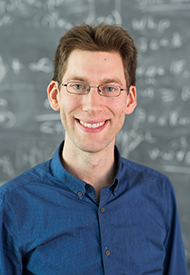
\includegraphics[width=3cm]{harrow_aram.jpg}
\caption{Aram W. Harrow (MIT, Boston)}
\end{figure}

\begin{small}
According to \cite{Aaronson2015}, the algorithm at the center of the "quantum machine learning" mini-revolution is called HHL \cite{Harrow2009}.

But, existing quantum algorithms for optimization and machine learning are often less complete than their classical counterparts because they do not use realistic models of their input data.
\end{small}
\end{frame}

\begin{frame}{Quantum Algorithm Models}
\protect\hypertarget{quantum-algorithm-models}{}
\vspace{0.5cm}
\begin{block}{~\vspace{0.7cm}}
\begin{table}
\scriptsize
\begin{center}
\vspace{-0.7cm}
\begin{tabular}{c | c | c}
  \thead{\textcolor{white}{\bf Model}} & \thead{\textcolor{white}{\bf Definition}} & \thead{\textcolor{white}{\bf Example}}  \\
  \makecell{Standard} &
  \makecell{Input $x \in {0, 1}^n$ \\ Output: $y \in {0, 1}$ }  &
  \makecell{factoring / number theory \\ combinatorial optimization}
  \\
  \hline
  Oracle &
  \makecell{given access to $O$ \\ $O \left|i, a \right\rangle = \left|i, a + x_i \right\rangle $} &
  \makecell{Grover, NAND tree, collision, ...\\ Hidden subgroup problem, welded trees} \\
  \hline
  Quantum Data &
  given state $\left|\psi \right\rangle$ &
  \makecell{QFT \\ SWAP test, Schur transform \\ tomography \\ linear systems } \\
  \hline
  Quantum Oracle & Given $U$ &
  \makecell{phase estimation\\ quantum sensing, process tomography\\qubitization, singular value transform}\\
\end{tabular}
\end{center}
\end{table}
\end{block}
\end{frame}

\begin{frame}{Quantum Search}
\protect\hypertarget{quantum-search}{}
\begin{columns}[T]
\begin{column}{.5\textwidth}

\begin{figure}
\centering
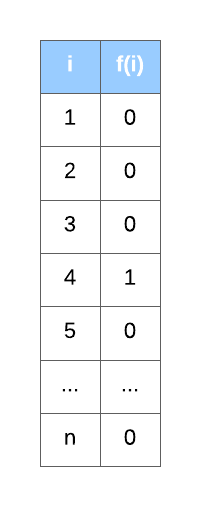
\includegraphics[width=2cm]{search.png}
\end{figure}
\end{column}

\begin{column}{.5\textwidth}

\begin{block}{}

Given the ability to compute $f(i) := x_i$

Find $i^*$ such that $f(i*) = 1$
\end{block}

\textbf{Classical}: $\mathcal{O}(n)$ time needed

\pause

\textbf{Grover's algorithm \cite{Grover96}}: (1996)

$\mathcal{O}(\sqrt{n})$ on quantum computer

\end{column}
\end{columns}

\pause

\textbf{similar speedups} for maximizing, approximate counting,
collisions, triangle finding, game-tree evaluation, sampling,
backtracking algorithms, rapidly mixing Markov chains
\end{frame}

\begin{frame}{Oracle search?}
\protect\hypertarget{oracle-search}{}
\begin{columns}[T]

\begin{column}{.1\textwidth}
\vspace{0.1cm}
usual

model
\end{column}

\begin{column}{.4\textwidth}
\begin{tcolorbox}[minipage,colback=white,arc=0pt,outer arc=0pt, boxsep=-2pt]
\centering
"oracle" = subroutine 

$O \lvert i \rangle \lvert 0 \rangle = \lvert i \rangle \lvert x_i \rangle$
\end{tcolorbox}
\end{column}

\pause

\begin{column}{.1\textwidth}
\vspace{0.5cm}
\centering
$\Rightarrow$

\end{column}
\begin{column}{.4\textwidth}
\vspace{0.1cm}
provable speedups,
sometimes exponential
\end{column}

\end{columns}

\pause

\begin{block}{\textbf{However}}
\protect\hypertarget{section-1}{}
\begin{itemize}
\item
  We cannot query a data center in superposition
\item
  Classical memory is \(\approx\) parallel.

  For large enough \(n\), \(n\) bits of memory \(\leftrightarrow\)
  \(\mathcal{O}(n)\) CPUs.
\item
  Proposed ``quantum RAM'' could be queried in superposition, but not
  easy to build.
\end{itemize}
\end{block}
\end{frame}

\begin{frame}{Oracles from classical memory}
\protect\hypertarget{oracles-from-classical-memory}{}
\begin{columns}[T]
\begin{column}{.4\textwidth}

\begin{figure}
\centering
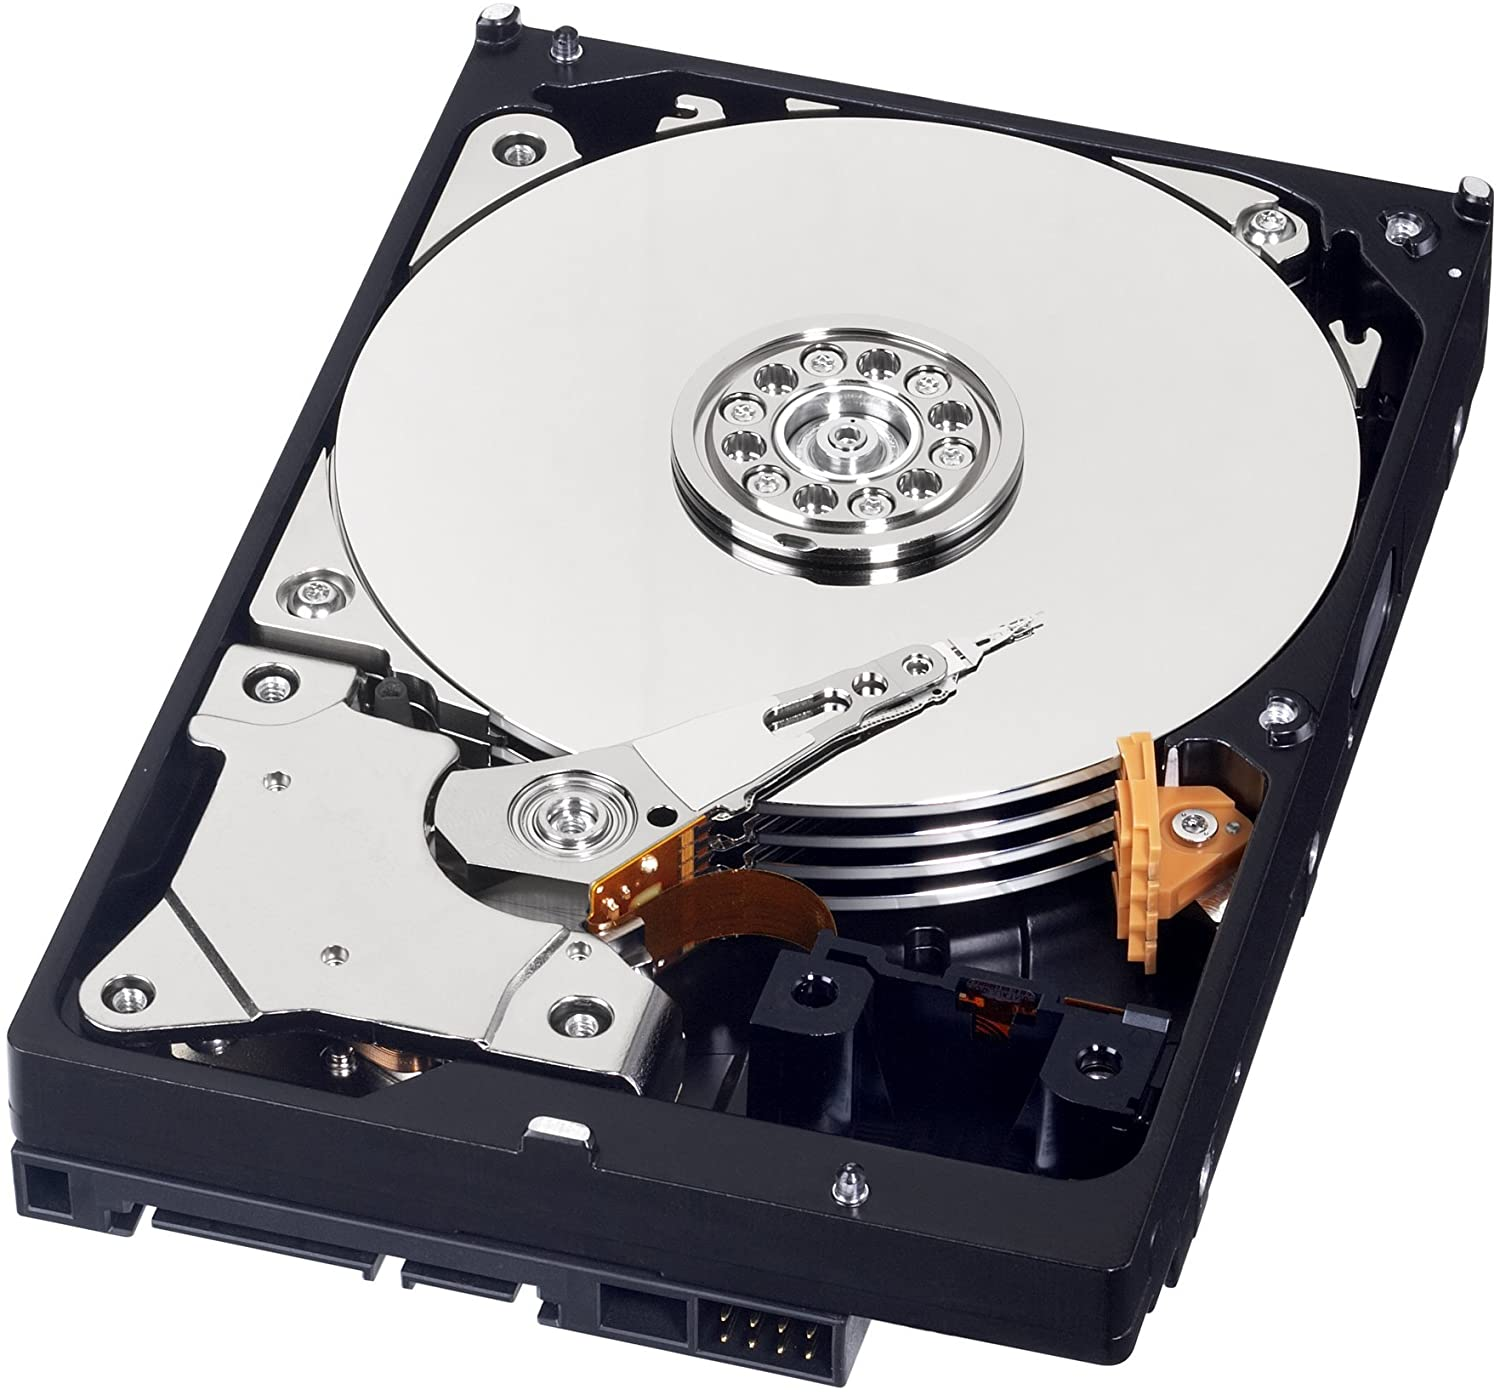
\includegraphics[height=2.5cm]{hard_drive.jpg}
\caption{$x_1, ..., x_n$}
\end{figure}

\end{column}
\begin{column}{.1\textwidth}
\pause
\begin{center}
\vspace{1.5cm}
$\Rightarrow$
\end{center}
\end{column}

\begin{column}{.4\textwidth}
\begin{figure}
\centering
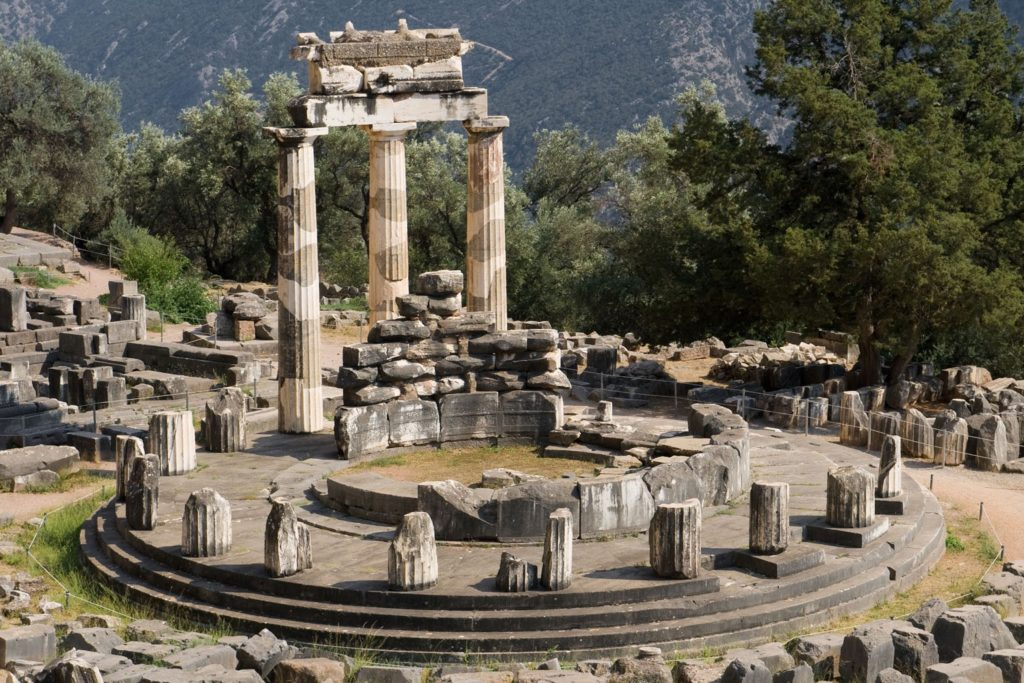
\includegraphics[height=2.5cm]{oracle.jpg}
\caption{$O \lvert i \rangle \lvert 0 \rangle = \lvert i \rangle \lvert x_i \rangle$}
\end{figure}
\end{column}

\end{columns}

\pause

\begin{figure}
\centering
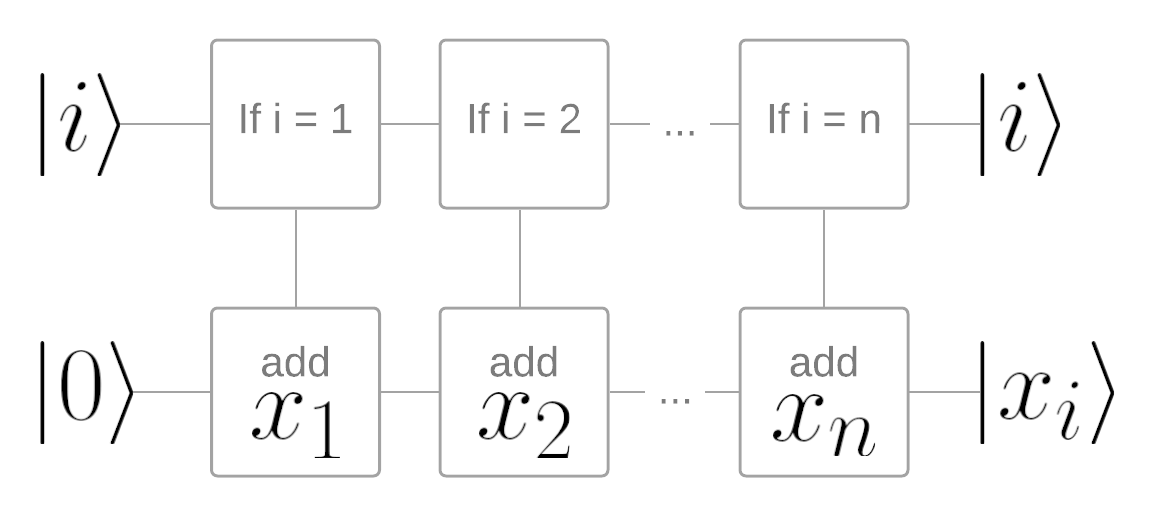
\includegraphics[height=3.2cm]{RAM.png}
\end{figure}
\end{frame}

\begin{frame}{Big data quantum speedups}
\protect\hypertarget{big-data-quantum-speedups}{}
Queries with overhead \(\mathcal{O}(n)\) mean no oracle speedup.

\pause

\begin{block}{Usual solutions}
\protect\hypertarget{usual-solutions}{}
\begin{enumerate}
\tightlist
\item
  QRAM: quantumly-accesible database
\item
  \(x_i = f(i)\) for efficient \(f\), e.g.~\(f(i) = a^i mod N\).
\end{enumerate}

\pause
\end{block}

\begin{block}{New approach}
\protect\hypertarget{new-approach}{}
Find problems where we can reduce the size of the data set

\begin{itemize}
\tightlist
\item
  Clustering
\item
  Bayesian Inference
\item
  Saddle-Point optimization
\end{itemize}
\end{block}
\end{frame}

\hypertarget{statistics-using-data}{%
\section{Statistics using data}\label{statistics-using-data}}

\begin{frame}{}
\protect\hypertarget{section-2}{}
\begin{block}{Maximum-likelihood estimation:}
\protect\hypertarget{maximum-likelihood-estimation}{}
\begin{small}

Given a set of models $Y$ and a data set $X$

Compute $\max \limits_{y} [ r(y) + \sum_{x \in X} f(x, y) ]$

Where $f(x, y) = \log p(x | y)$.

\end{small}
\end{block}

\pause

\begin{block}{}
\protect\hypertarget{section-3}{}
\begin{small}

$\mathbf{X, Y}$ appear almost symmetrically. ($\max vs \sum$ don't matter for Grover)

but

$X$ lives on a \textbf{hard drive} $\rightarrow$ \textbf{no oracle access or superposition}

$Y$ is \textbf{synthetic} (e.g weights and centers of clusters) $\rightarrow$ \textbf{can superpose}

\end{small}
\end{block}

\pause

\begin{block}{}
\protect\hypertarget{section-4}{}
\begin{small}
Classical computer controlling a quantum computer:
Can run Grover with $\mathcal{O}{(\left|X\right| \cdot \left|Y\right|^{1/2})}$
\end{small}
\end{block}

\centering

Key question: Can we reduce the dependence on \(\left|X\right|\) ?
\end{frame}

\hypertarget{data-reduction}{%
\section{Data Reduction}\label{data-reduction}}

\begin{frame}{Coresets}
\protect\hypertarget{coresets}{}
\begin{columns}[T]
\begin{column}{.4\textwidth}

\begin{figure}
\centering
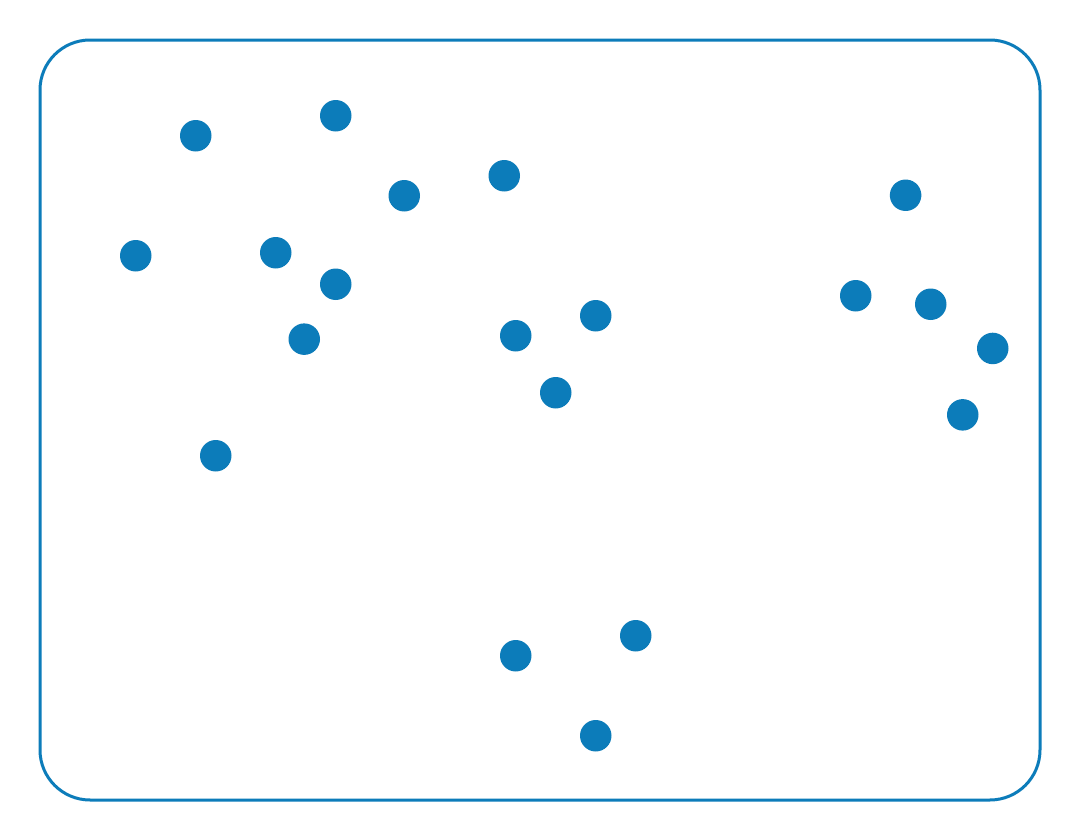
\includegraphics[width=1\textwidth]{dataset.png}
\caption{$X$}
\end{figure}

\end{column}
\begin{column}{.1\textwidth}
\pause
\begin{center}
\vspace{1.5cm}
$\Rightarrow$
\end{center}
\end{column}

\begin{column}{.4\textwidth}
\begin{figure}
\centering
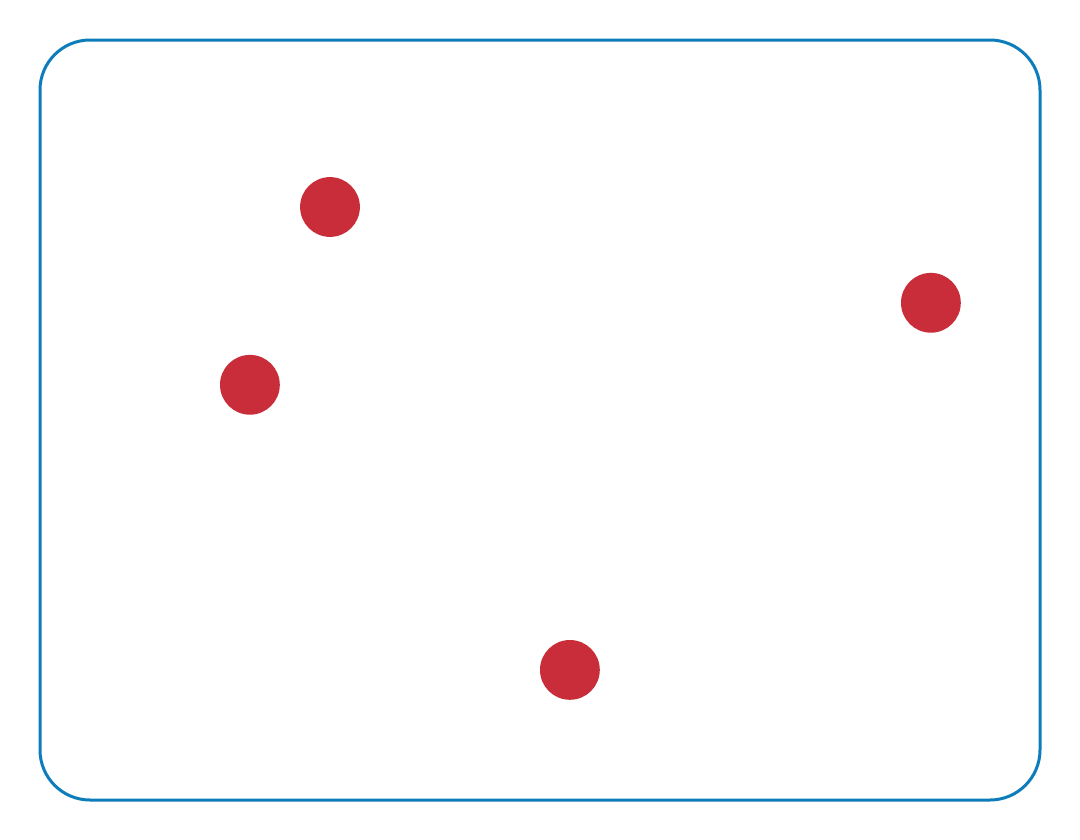
\includegraphics[width=1\textwidth]{coreset.png}
\caption{$X'$}
\end{figure}
\end{column}

\end{columns}

\pause

\begin{block}{}
\protect\hypertarget{section-5}{}
\(X'\) is a \textbf{coreset} if for all \(y\),

\(\sum_{x \in X} f(x, y) \approx \sum_{x \in X'} w(x) f(x, y)\)
\end{block}
\end{frame}

\begin{frame}{Hybrid algorithms for machine learning}
\protect\hypertarget{hybrid-algorithms-for-machine-learning}{}
\begin{center}
$X \rightarrow$ \fbox{classical computer} $\underrightarrow{X'}$ \fbox{quantum computer} $\rightarrow y$
\end{center}

\begin{columns}
\begin{small}
\begin{column}{.5\textwidth}

\begin{itemize}
\item Finds quick, crude guess of $y'$.
\item Use $y'$ to construct importance sampling weights
\item Draw $X'$ using importance sampling.
\end{itemize}

\end{column}
\begin{column}{.5\textwidth}

\begin{itemize}
\item Use Grover / q walks / adiabatic / etc to find $y$.
\item Inner loop cost is $\mathcal{O}(\left|X'\right|)$ \\ Total cost for Grover $\mathcal{O}(\left|X'\right| \cdot \left|Y\right|^{\frac12})$
\item Provable speedups include clustering.
\end{itemize}

\end{column}
\end{small}
\end{columns}
\end{frame}

\begin{frame}{Importance sampling}
\protect\hypertarget{importance-sampling}{}
\begin{columns}[T]
\begin{column}{.2\textwidth}
\begin{figure}
\centering
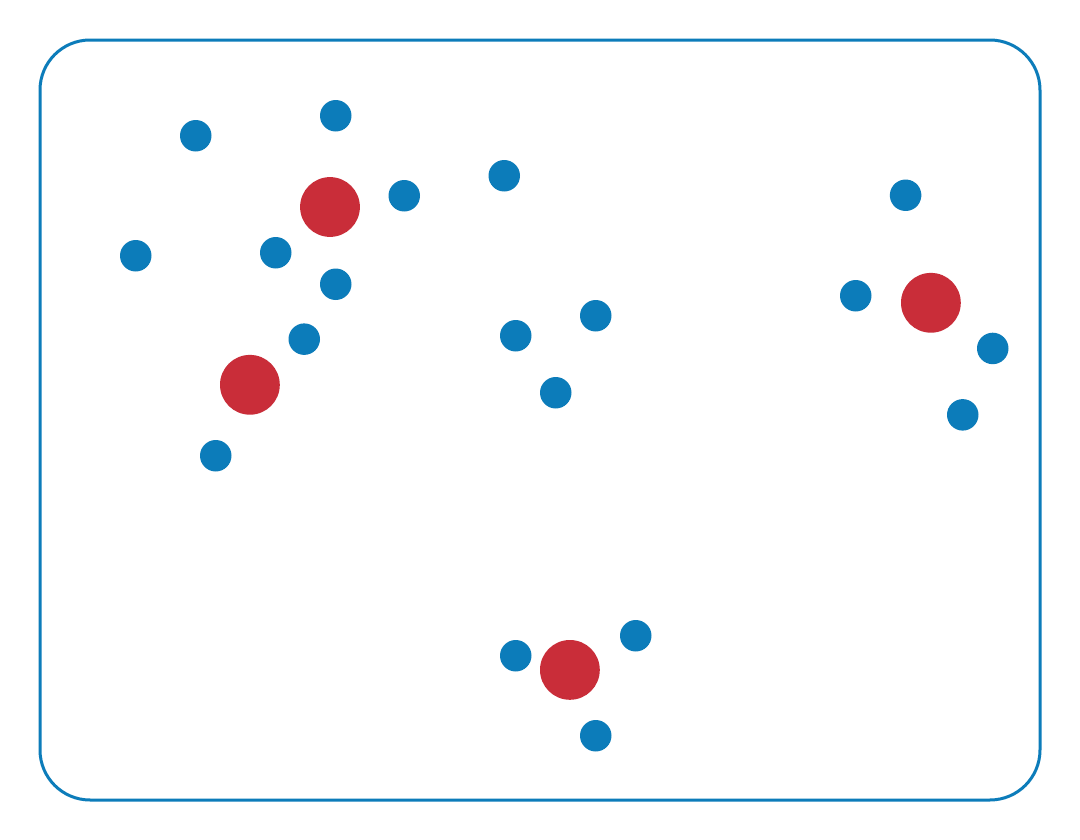
\includegraphics[width=1\textwidth]{data-core-set.png}
\caption{$X'$}
\end{figure}
\end{column}
\begin{column}{.8\textwidth}
\begin{small}
\textbf{Goal:} for all y,  $\sum_{x \in X} f(x, y) \approx \sum_{x \in X'} w(x) f(x, y)$
\pause
\textbf{Challenges}

1. X' estimator should be unbiased

2. For any fixed y, need to control the variance $$\sigma^2 = E_x [f(x, y)^2] - E_x[f(x, y)]^2$$

3. X' needs to work simultaneously for all y.

\end{small}
\end{column}
\end{columns}
\pause

\textbf{Solutions}

\begin{enumerate}
\tightlist
\item
  Sample \(x\) with probability \(\propto s(x)\). Assign weight
  \(\propto \frac{1}{s(x)}\)
\item
  Importance Sampling: Choose
  \(s(x) \geq max_{y} [\frac{f(x, y)}{\sum_{x'} f(x', y)}]\)
\item
  Bound pseudo-dimension D of family \(f(., y)\).
\end{enumerate}
\end{frame}

\begin{frame}{Non-adaptive coresets}
\protect\hypertarget{non-adaptive-coresets}{}
\vspace{0.2cm}
\begin{columns}[T]
\begin{column}{.55\textwidth}
\vspace{-0.5cm}
\begin{block}{}
\begin{small}
\textbf{Thm:} Importance sampling $x_1, ..., x_m$

yields a $\epsilon-coreset$ with prob. $\geq 1 - \delta$ if 

$$m \gtrsim \frac{S^2}{\epsilon^2} \left (D + \log \frac{1}{\delta} \right) $$

\end{small}
\end{block}
\end{column}
\begin{column}{.45\textwidth}
\begin{small}
Given:

$s(x) \geq max_{y} [\frac{f(x, y)}{\sum_{x'} f(x', y)}]$.

total sensitivity $S = \sum_x s(x)$.

Pseudo dimesion $D$.
\end{small}
\end{column}
\end{columns}

\vspace{0.5cm}
\begin{columns}[T]
\begin{column}{.6\textwidth}
\pause
\begin{small}
\textbf{Example: k-means in} $R^d$

$y = (y^{(1)}, ..., y^{(k)})$ = positions of $k$ centers.

$f(x,y) = -\min_j dist(x, y^{(j)})^2$

pseudo-dim: D = $\mathcal{O}(d k \log(k))$

sensitivity: $S \leq \mathcal{O}(k)$
\end{small}
\end{column}
\pause
\begin{column}{.4\textwidth}
\vspace{1cm}
$\Rightarrow m \gtrsim \frac{dk^3 \log k + k^2 \log {\frac{1}{\delta}}}{\epsilon^2}$
\end{column}
\end{columns}

\pause

\begin{block}{Algorithm}
\protect\hypertarget{algorithm}{}
\begin{small}
1. Classical computer finds $s(x)$ for each $x \in X$ and samples $x_1, ..., x_m$

2. Brute force search in time $k^m$ classical or $k^{\frac{m}{2}}$ quantumly

(Or use other algorithms, like adiabatic, quantum walks, etc..)
\end{small}
\end{block}
\end{frame}

\begin{frame}{Adaptive data-reduction}
\protect\hypertarget{adaptive-data-reduction}{}
\begin{center}
$X \rightarrow$ \fbox{classical computer} $\underrightarrow{X'}$ \fbox{quantum computer} $\rightarrow y$
\end{center}

Data set is small by the time we turn the quantum computer.

\pause

\begin{columns}[T]
\begin{column}{.05\textwidth}
\vspace{0.6cm}
\centering
$X$
\end{column}
\begin{column}{.05\textwidth}
\vspace{0.7cm}
\centering
$\rightarrow$
\end{column}

\begin{column}{.375\textwidth}
\begin{block}{}
\centering
classical 

computer
\end{block}
\end{column}

\begin{column}{.05\textwidth}
\vspace{0.3cm}
\centering

$\rightarrow$

\vspace{-0.3cm}

$\leftarrow$

\vspace{-0.3cm}
...
\vspace{-0.2cm}

$\rightarrow$

\vspace{-0.2cm}

$\leftarrow$

\end{column}

\begin{column}{.375\textwidth}
\begin{block}{}
\centering
quantum

computer
\end{block}
\end{column}

\begin{column}{.05\textwidth}
\vspace{0.7cm}
\centering
$\rightarrow$
\end{column}


\begin{column}{.05\textwidth}
\vspace{0.6cm}
\centering
$y$
\end{column}
\end{columns}

Are there benefits to using the quantum computer interactively?
\end{frame}

\begin{frame}{Adapative coresets}
\protect\hypertarget{adapative-coresets}{}
\begin{footnotesize}
[Campbell, Broderick 2017] [Bugalo, Elvira, Martino, Luengo, Míguez, Djuric, 2017]
\end{footnotesize}

Bayesian Inference: sample \(y\) from:

\(\pi(y) = \frac{\pi_{0}(y) \exp{\sum_{x \in X} f(x, y)} } {Z}\)

\pause

\begin{columns}[T]

\begin{column}{.325\textwidth}
\begin{block}{}
\vspace{0.2cm}
\centering
classical 

computer
\vspace{0.2cm}
\end{block}
\end{column}

\begin{column}{.35\textwidth}
\vspace{0.4cm}
\centering
\begin{small}
data $x_1, ..., x_t$

weights $w(x_1), ..., w(x_t)$

\end{small}


$\longrightarrow$

\vspace{-0.2cm}

$\longleftarrow$
\end{column}

\begin{column}{.325\textwidth}
\begin{block}{}
\vspace{0.2cm}
\centering
quantum

computer
\vspace{0.2cm}
\end{block}
\end{column}

\end{columns}

\pause

Sample \(y_t\) from
\(\pi_t(y_t) = \frac{\pi_{0}(y) \exp{\sum_{i=1}^{t} w(x_i) f(x_i, y)} } {Z}\)

\pause

Choose \(x_{t+1}, w(x_{t+1})\) using
\(y_1, ..., y_t, x_1, ..., x_t, w(x_1), ..., w(x_t)\)
\end{frame}

\begin{frame}{Comparison with variational algorithms}
\protect\hypertarget{comparison-with-variational-algorithms}{}
\begin{small}

1. Variational algorithms use a classical outer loop to perform gradient descent on the circuit parameters of a quantum inner loop.  These can be extremely generaland in some cases amount to performing a local search over the set of all short circuits implementable in a particular hardware model.  As a result, they often lack the provable guarantees of algorithms in this paper.  On the other hand, they can be run on even very simple quantum computers and running them can teach us about what we might expect from future quantum hardware.

2. There are two key features of our Algorithm 3 that are not suggested by the usual variational formulation:  1) the ansatz and the classical outer loopare structured carefully to present the quantum computer with a very limited subset of the overalldata set,  and;  2) the output of the quantum computer is usable for a form of stochastic mirror descent without any of the dimension dependence that is seen in general (e.g [36]).

\end{small}
\end{frame}

\begin{frame}{Comparison with stochastic gradient descent}
\protect\hypertarget{comparison-with-stochastic-gradient-descent}{}
\begin{small}

1. The essential difference between SGD and coresets is that coresets are sampled once and then used  throughout  the  optimization,  while  SGD  draws  fresh  samples  for  each  gradient  step.   For classical gradient descent,  this difference may not be important,  or it may favor SGD. However, when used as a subroutine inside a Grover or Durr-Høyer search, the stochastic noise introduced by SGD can be harmful.  Indeed, the Grover speedup is known to vanish when the oracle is stochastic and has a non-negligible chance of being replaced by the identity operator [49].

\end{small}
\end{frame}

\begin{frame}{Comparison with stochastic gradient descent}
\protect\hypertarget{comparison-with-stochastic-gradient-descent-1}{}
\begin{small}

2.  This is an example of a more general problem.  A subset of size $k$, whether used as a coreset ora SGD minibatch, may be “bad” with probability $\delta$.  For coreset algorithms this means the overall algorithm fails with probability $\delta$.  For a Grover search using SGD, this means the overall algorithm fails with probability  $\sqrt{|Y|} \delta$.  (Other algorithms for searching over Y, such as the adiabatic algorithm, may have a more complicated dependence on stochastic noise, and studying this difference is an important open question.)

3. Recently there has been enormous progress in our theoretical and practical understanding of more sophisticated variants of gradient descent [52], and it is an important open question to un-derstand what potential these have for benefiting quantum algorithms.

\end{small}
\end{frame}

\begin{frame}{Perspective}
\protect\hypertarget{perspective}{}
\begin{enumerate}
\item
  Grover is used for concreteness but same ideas apply to adiabatic
  algorithm, QAOA, quantum walks, etc.
\item
  QCs will augment not replace classical computers. Let's design
  algorithms as though we believe this!
\end{enumerate}
\end{frame}

\hypertarget{recent-work}{%
\section{Recent Work}\label{recent-work}}

\begin{frame}{Coreset Clustering on Small Quantum Computers
\cite{tomesh2020coreset}}
\protect\hypertarget{coreset-clustering-on-small-quantum-computers}{}
\begin{small}
Many quantum algorithms for machine learning require access to classical data in superposition. However, for many natural data sets and algorithms, the overhead required to load the data set in superposition can erase any potential quantum speedup over classical algorithms. Recent work by Harrow introduces a new paradigm in hybrid quantum-classical computing to address this issue, relying on coresets to minimize the data loading overhead of quantum algorithms. We investigate using this paradigm to perform k-means clustering on near-term quantum computers, by casting it as a QAOA optimization instance over a small coreset. We compare the performance of this approach to classical k-means clustering both numerically and experimentally on IBM Q hardware. We are able to find data sets where coresets work well relative to random sampling and where QAOA could potentially outperform standard k-means on a coreset. However, finding data sets where both coresets and QAOA work well--which is necessary for a quantum advantage over k-means on the entire data set--appears to be challenging.

\end{small}
\end{frame}

\begin{frame}{A hybrid classical-quantum workflow for natural language
processing \cite{ORiordan2020AHC}}
\protect\hypertarget{a-hybrid-classical-quantum-workflow-for-natural-language-processing}{}
\begin{small}
Natural language processing (NLP) problems are ubiquitous in classical computing, where they often require significant computational resources to infer sentence meanings. With the appearance of quantum computing hardware and simulators, it is worth developing methods to examine such problems on these platforms. In this manuscript we demonstrate the use of quantum computing models to perform NLP tasks, where we represent corpus meanings, and perform comparisons between sentences of a given structure. We develop a hybrid workflow for representing small and large scale corpus data sets to be encoded, processed, and decoded using a quantum circuit model. In addition, we provide our results showing the efficacy of the method, and release our developed toolkit as an open software suite.

\end{small}
\end{frame}

\begin{frame}{}
\protect\hypertarget{section-6}{}
\begin{Huge}
Thanks!
\end{Huge}
\end{frame}

\begin{frame}[allowframebreaks]{}
  \bibliographytrue
  \printbibliography[heading=none]
\end{frame}

\end{document}
